\documentclass{article}
\usepackage[utf8]{inputenc}
\usepackage[spanish]{babel}
\usepackage{graphicx}
\usepackage{float}
\usepackage{amsmath}
\usepackage{listings}
\usepackage{xcolor}

\definecolor{codegreen}{rgb}{0,0.6,0}
\definecolor{codegray}{rgb}{0.5,0.5,0.5}
\definecolor{codepurple}{rgb}{0.58,0,0.82}
\definecolor{backcolour}{rgb}{0.95,0.95,0.92}

\lstdefinestyle{mystyle}{
	backgroundcolor=\color{backcolour},   
	commentstyle=\color{codegreen},
	keywordstyle=\color{magenta},
	numberstyle=\tiny\color{codegray},
	stringstyle=\color{codepurple},
	basicstyle=\ttfamily\footnotesize,
	breakatwhitespace=false,         
	breaklines=true,                 
	captionpos=b,                    
	keepspaces=true,                 
	numbers=left,                    
	numbersep=5pt,                  
	showspaces=false,                
	showstringspaces=false,
	showtabs=false,                  
	tabsize=2
}

\lstset{style=mystyle}

% Title Page
\title{Simulación de la trayectoria de un cohete mediante la resolución de un sistema de ecuaciones diferenciales usando el método de Runge-Kutta de orden 4}
\author{Rodrigo P.,Eduardo C.,Carmen R.}
\date{24 de mayo de 2020}

\begin{document}
\maketitle

\begin{abstract}
	En el presente artículo se muestra la resolución de un problema de mecánica planetaria mediante la resolución numérica de un sistema de cuatro ecuaciones diferenciales haciendo uso de un programa en C++ y el método de Runge-Kutta de cuarto orden. Con la resolución de este sistema de ecuaciones se pretende encontrar la trayectoria que sigue una nave espacial en un viaje translunar bajo la influencia gravitatoria de la tierra y la luna. Las variables involucradas en el sistema de ecuaciones son el radio, el ángulo polar y los momentos generalizados de la nave en un instante del tiempo dado, se programó una función contenedora para el sistema de ecuaciones haciendo uso de estas variables y posteriormente se evaluó haciendo uso del método RK4, los resultados se guardaron en un archivo de texto.Los resultados arrojaron que el tiempo necesario para intersectar la trayectoria lunar es aproximadamente un dia con una velocidad cercana a la velocidad de escape de la tierra y un ángulo de 65 grados, estos resultados son congruentes con la realidad por lo que la resolución del sistema de ecuaciones fue exitosa
\end{abstract}

\section{Planteamiento}

El problema consiste en modelar la trayectoria de un cohete bajo la influencia gravitacional de la luna y la tierra,para ello es necesario ubicar a la nave en el espacio, esto se hace con el uso de las coordenadas $r$ y $\phi$. La luna se mueve en una órbita circular de radio $r_1$ con frecuencia constante $\omega$ al rededor de la tierra.\\

\begin{figure}[H]
	\centering
	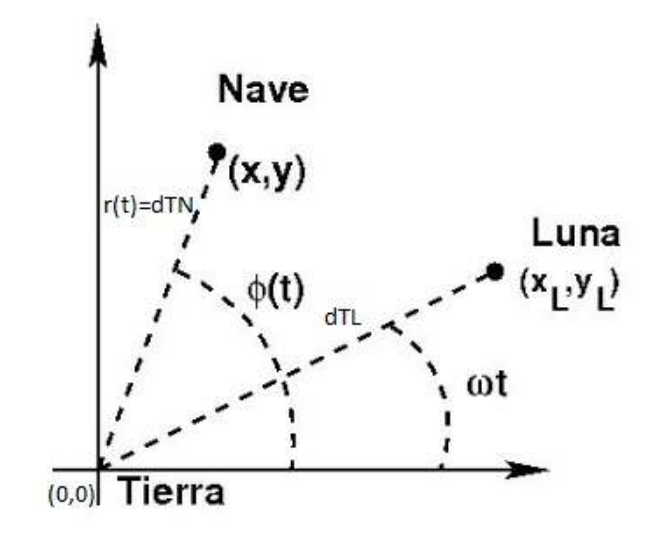
\includegraphics[width=8cm]{Sistema}
	\caption{Ubicación de la nave y la luna en el espacio.}
\end{figure}

El movimiento de este sistema está descrito por un sistema de cuatro ecuaciones diferenciales de primer orden$^{[1]}$ donde las variables son: $\bar{r}$, $\phi$, $\bar{p_r}$ y $\bar{p_{\phi}}$

\begin{align}
\frac{d\bar{r}}{dt}=\bar{p_r}\\
\frac{d\phi}{dt}=\frac{\bar{p_{\phi}}}{\bar{r}^2}\\
\frac{d\bar{p_r}}{dt}=\frac{\bar{p_{\phi}}^2}{\bar{r}^3}-\Delta\left[ \frac{1}{\bar{r}^2} +\frac{\mu}{\bar{r'}^3}[\bar{r}-cos(\phi -\omega t)]\right]\\
\frac{d\bar{p_{\phi}}}{dt}=-\frac{\Delta \mu \bar{r}}{\bar{r'}^3}sin(\phi -\omega t)
\end{align}

Donde:
\begin{align*}
\Delta = \frac{GM_T}{r^3_l}\\
\mu = \frac{M_T}{M_l}\\
\bar{r'}=\sqrt{1+\bar{r}^2-2\bar{r}cos(\phi-\omega t)}
\end{align*}

Las variables del sistema de ecuaciones están ajustadas para ser adimensionales o tener unidades de 1/s, de esta forma, $\bar{r}$ está relacionada a la distancia radial de la nave al centro del sistema coordenado, $\phi$ es el ángulo de desfase entre la luna y la tierra y $\bar{p_r}$, $\bar{p_{\phi}}$ están relacionadas con los momentos generalizados de la nave en la dirección radial y angular, en términos de variables físicas se definen de la siguiente forma:
\begin{align*}
\bar{r} = r/r_l\\
\phi =\phi\\
\bar{p_r} = \frac{v}{r_l}cos(\theta-\phi)\\
\bar{p_{\phi}}=\frac{rv}{r^2_l}sin(\theta-\phi)\\
\end{align*}

Donde $\theta$ es el ángulo que forma el vector momento con el vector radial de la posición de la nave
\begin{figure}[H]
	\centering
	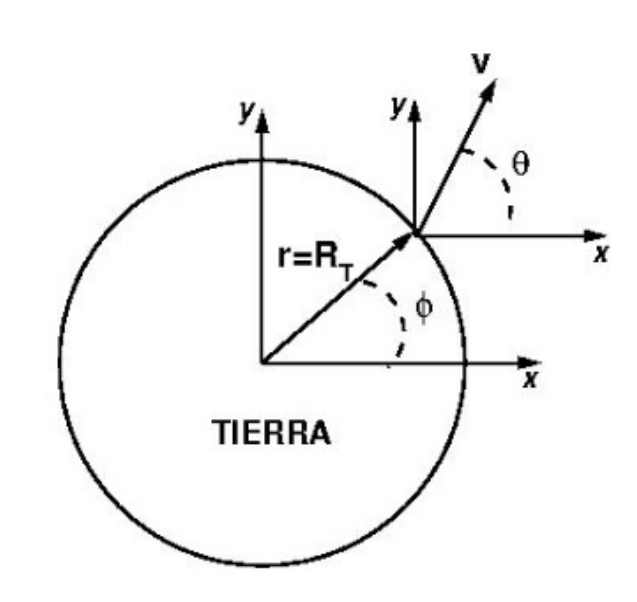
\includegraphics[width=8cm]{Nave-Tierra}
	\caption{Ilustración de la ubicación de los ángulos $\phi$ y $\theta$}
\end{figure}

\section{Metodología}

La resolución numérica del sistema de ecuaciones diferenciales se hizo mediante el método de Runge-Kutta de orden 4, para ello se proporcionaron 4 condiciones iniciales siendo estas las siguientes:

\begin{align*}
\bar{r_0} = r_T/r_l =0.01659\\
\theta =65\degres\\
\phi =0\\
\bar{v_0}=v_0/r_l =2.9338\times 10^{-5} 1/s\\
\bar{p_r} = \bar{v_0}cos(\theta-\phi)\\
\bar{p_{\phi}}=\frac{r_0v_0}{r^2_l}sin(\theta-\phi)
\end{align*}

Se usó un programa para evaluar el método continuamente 43,200 veces con un paso de 2s, haciendo que la simulación evaluara un tiempo total de 24 horas de movimiento, el programa fué hecho en C++ y evaluado para este sistema de ecuaciones en particular.

Las funciones del sistema de ecuaciones fueron condensadas en una sola función contenedora que devolvía una evaluación distinta dependiendo del parámetro que se le indicase
\pagebreak

\begin{lstlisting}[language=C++,caption=código de la función condensadora del sistema de ecuaciones]
double f(double t, double* xi, int n){
double fr;
const double om =2.6617e-6, delta  =7.014e-12, mu =0.0123;
double r = xi[0], phi = xi[1], pr = xi[2], pp = xi[3];
double rpr = sqrt(1+r*r-2*r*cos(phi - om*t));
switch (n){
case 0:
fr = pr;
break;
case 1:
fr= pp/(r*r);
break;
case 2:
fr = (pr*pr)/(r*r*r)*delta*(1.0/(r*r)+(r-cos(phi - om*t))*mu/(rpr*rpr*rpr));
break;
case 3:
fr=-sin(phi - om*t)*delta*mu*r/(rpr*rpr*rpr);
break;
}
return fr;
}
\end{lstlisting}

Esta función se usó para evaluar el método RK4 para sistemas de ecuaciones dadas las condiciones iniciales y los resultados se escribieron en un archivo de texto:

\begin{lstlisting}[language=C++,caption=Aplicación del método RK4 y escritura en un archivo de texto]
void RK4sys(double ti,double* xi,double f(double t, double* xi, int n),double h, const int n, const int m){
double x[n]={};
double t = ti;
for (int i = 0;i<n;i++){
x[i]=xi[i];
}

ofstream file("datos.dat");
file << setprecision(8);
for (int j = 0;j<m;j++){
file << t<<" "; 
for (int i = 0;i<n;i++){ 
file << x[i]<<" ";
x[i]=xvnext(t,x,f,h,n)[i];     
} 
t = t +h;
file << endl;
}
}
\end{lstlisting}

El método RK4 en sí se encuentra en la función "xvnext", esta toma un estado y una función y devuelve el siguiente estado al avanzar un paso.

\begin{lstlisting}[language=C++,caption=Método RK4 para sistemas de ecuaciones diferenciales]
double* xvnext(double t,double* xi,double f(double t, double* xi, int n),double h, const int n){
double k1[n]={};
double k2[n]={};
double k3[n]={};
double k4[n]={};
double* xs = new double[n];

for (int i = 0;i<n;i++){
k1[i]=f(t,xi,i);
xs[i] = xi[i] + k1[i]*h/2.0;
}
for (int i = 0;i<n;i++){
k2[i] = f(t+h/2.0,xs,i);
xs[i] = xi[i] + k2[i]*h/2.0;
}
for (int i = 0;i<n;i++){
k3[i] = f(t+h/2.0,xs,i);
xs[i] = xi[i] + k3[i]*h;
}
for (int i = 0;i<n;i++){
k4[i] = f(t+h,xs,i);
}
for (int i = 0;i<n;i++){
xs[i] = xi[i]+h*(k1[i]+2*k2[i]+2*k3[i]+k4[i])/6.0;
}
return xs;
}
\end{lstlisting}

\section{Resultados}

Haciendo uso del programa antes descrito se obtuvo una lista de 43,200 estados del sistema, es decir, los valores de cada variable en un dado instante de tiempo, las variables $\bar{r}$ y $\phi$ dictan la trayectoria del cohete, estas se graficaron de forma polar junto a la trayectoria de la luna, se obtuvo lo siguiente:

\begin{figure}[H]
	\centering
	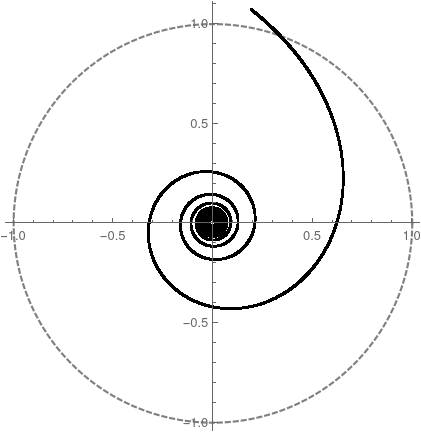
\includegraphics[width=8cm]{Trayectoria}
	\caption{Trayectoria obtenida de la nave (negro) y trayectoria de la luna (gris)}
\end{figure}

Esta gráfica está normalizada respecto al radio de la luna, se puede notar que la trayectoria del cohete intersecta a la de la luna en aproximadamente 1 dia y la trayectoria es espiraloide.
\section{Conclusiones}
Se obtuvo satisfactoriamente la solución al sistema de ecuaciones propuesto y por consiguiente la trayectoria de la nave bajo la influencia de la gravedad de la tierra y la luna.
Se puede notar que el tiempo para intersectar la trayectoria lunar es aproximadamente un día con una velocidad inicial cercana a la velocidad de escape de la tierra, este resultado coincide con la realidad y es congruente con la duración de los viajes reales a la luna.
La resolución de este método puede ser aplicado para encontrar trayectorias reales de vuelo translunar y ser adaptado para encontrar trayectorias de viaje transplanetario de igual forma.

\begin{thebibliography}{1}
	
	\bibitem{latexcompanion} 
	Ivón Fabian,  
	\textit{Modelado y simulación del movimiento de un cohete mediante un sistema de ecuaciones diferenciales}. 
	Universidad autónoma del estado de México, Toluca, 2019.
\end{thebibliography}

\end{document}          
